% Preamble
%\documentclass[xetex,mathserif,serif]{beamer}
\documentclass{beamer}

% Packages
\usepackage[spanish]{babel}
\selectlanguage{spanish}
\usepackage[utf8]{inputenc} % For spanish (and international) letters like acents.
\usepackage{hyperref} % To create hyperlinks within the document.
\usepackage{graphicx} % To include graphics (pictures, images)
\usepackage{float} % For the use of the parameter "H" in command "\begin{figure}[H]" (i.e. exact position of image in text)
\usepackage{verbatim} % For long comments
\usepackage{tikz} % For include Dia diagrams in .tex format

\graphicspath{{../Diagramas/}} % Path of the folder containing the images

\title{Colección Archivística del LAIS}
\subtitle{Sistema de apoyo a la catalogación de archivos audiovisuales}
\author{Rodrigo Colín Rivera, Sergio Amaro Rosas}
\institute
{
  Laboratorio Audiovisual de Investigación Social\\
  Instituto de Investigaciones Dr. José María Luis Mora
}
\date{\today}
\subject{Catalogación de Acervo Documental en Video}

\begin{comment}
\AtBeginSection[]
{
  \begin{frame}
    \frametitle{Tabla de contenidos}
    \tableofcontents[currentsection]
  \end{frame}
}
\AtBeginSubsection[]
{
  \begin{frame}
    \frametitle{Tabla de contenidos}
    \tableofcontents[currentsection,currentsubsection]
  \end{frame}
}
\end{comment}

% Style and theme
%\usetheme{Warsaw}
\usecolortheme{orchid} %crane,dolphin,lily

% Document environment
\begin{document}

\frame{\titlepage} % Página inicial

\section{Antecedentes y problemática actual}
\begin{frame}
	\frametitle{Introducción}
	El resguardo y documentación de materiales audiovisuales constituye una tarea prioritaria entre quienes recurrimos a ellos cotidianamente con fines de investigación. El Laboratorio Audiovisual de Investigación Social (LAIS) del Instituto de Investigación Dr. José María Luis Mora se propusó abocarse a esta labor para construir un acervo debidamente documentado, ponerlo en acceso para consulta y potenciar así la investigación con este tipo de materiales.
\end{frame}

\begin{frame}
	\frametitle{Antecedentes y problemática actual}
	El LAIS consta de una colección archivística para materiales audiovisuales cuyos registros actuales se encuentran en formato de \textbf{hojas de cálculo} (mediante Excel) que integran la ficha de documentación de cada material audiovisual.
	
	La problemática principal con esta manera de catalogación es que resulta \textbf{complicado buscar} o filtrar los registros. Además de otros problemas como La integridad de la información, la cantidad de usuarios que pueden consultar estos registro, la manipulación de los datos y el acceso a esta información.
\end{frame}

\section{Propuesta para el sistema de apoyo a la catalogación de archivos audiovisuales}
\begin{frame}
	\frametitle{Propuesta}
	\framesubtitle{Creación de un sistema computacional}
	
	La propuesta consiste en crear una \textbf{base de datos} para el manejo actual y futuro de las fichas de documentación de los materiales audiovisuales del LAIS junto con una \textbf{interfaz} de usuario que permita manipular fácilmente la base de datos.
\end{frame}

\subsection{Comparación entre hojas de cálculo y base de datos}
\begin{frame}[shrink]
	\frametitle{Propuesta}
	\framesubtitle{Comparaciones entre hojas de cálculo y base de datos}
	
	\begin{center}
		\begin{tabular}{| l | p{6.5cm} | p{6.5cm} |}
			\hline
			 & Hoja de cálculo & Base de datos \\ \hline
			 
			 Objetivo 
			 	& Realizar cálculos numéricos a través del uso de diversas fórmulas aritméticas. 
			 	& Almacenar datos en un servidor. \\
			 \hline
			 Almacenamiento
			 	& En archivos (libros) que contienen una o varias hojas de cálculo con filas y columnas para describir los datos.
			 	& En tablas que contienen registros (renglones) donde cada valor le corresponde un tipo de dato (columna)\\
			 \hline
			 Manejo
			 	& Cualquier persona con un conocimiento básico puede manipular, ordenar o filtrar datos.
			 	& Programador o persona encargada de la base de datos realiza consultas a través del lenguaje de programación SQL (\textit{Structured Query Language}). Requiere una interfaz de usuario para una fácil manipulación de la base. \\
			 \hline
			 Complejidad (datos)
			 	& Los datos son sencillos de manejar pero a mayor cantidad, mayor complejidad.
			 	& El modelo relacional permite mantener unidades organizadas para los datos (tablas) \\
			 	\hline
			 Repetición de datos
			 	& Se pueden presentar repetición o redundancia de datos.
			 	& Si el diseño de la base de datos es correcta, no se permite redundancia de información. \\
			 	\hline
			 Modificaciones
			 	& Una sola persona puede modificar a la vez. Varias personas con copia del original pueden hacer modificaciones pero al combinar la información queda sujeta a errores humanos.
			 	& Los manejadores (programas) de bases de datos permite multiusuarios y mecanismos de control en las modificaciones. \\
			 	\hline
			 Presentación
			 	& Adecuado para incrustar en documentos escritos o mostrar gráficas relativas a los datos contenidos.
			 	& Solamente a través de una interfaz de usuario se pueden presentar los datos. El formato varia según la implementación. \\
			 	\hline
		\end{tabular}
	\end{center}
\end{frame}

\section{Esquema general del sistema}
\begin{frame}
	\frametitle{Esquema general del sistema}
	Para la manipulación de la base de datos (consultar, buscar, insertar y borrar registros) se debe crear una interfaz intuitiva para los usuarios.
	La siguiente figura muestra el diseño general separando la \textbf{base de datos} de la \textbf{aplicación web} y mostrando las responsabilidades o usos de cada tipo de usuario (programador, interno del LAIS y usuario externo al LAIS).
\end{frame}

\begin{frame}
	\begin{figure}[H]
		\centering
		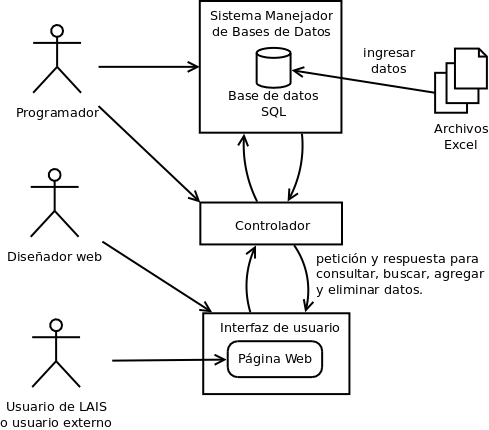
\includegraphics[width=0.8\textwidth]{EsquemaGeneral.png}
		\caption{Esquema general del sistema de consulta}
		\label{fig:esquema_general}
	\end{figure}
\end{frame}

\subsection{Casos de uso}
\begin{frame}
	\frametitle{Casos de uso}
	Los casos de uso son un tipo de diagrama que permite representar a los usuarios involucrados y las principales acciones del sistema.
	Las acciones básicas son: \textbf{consultar}, \textbf{buscar}, \textbf{agregar} y \textbf{editar} un material audiovisual.
\end{frame}

\begin{frame}
	\begin{figure}[H]
		\centering
		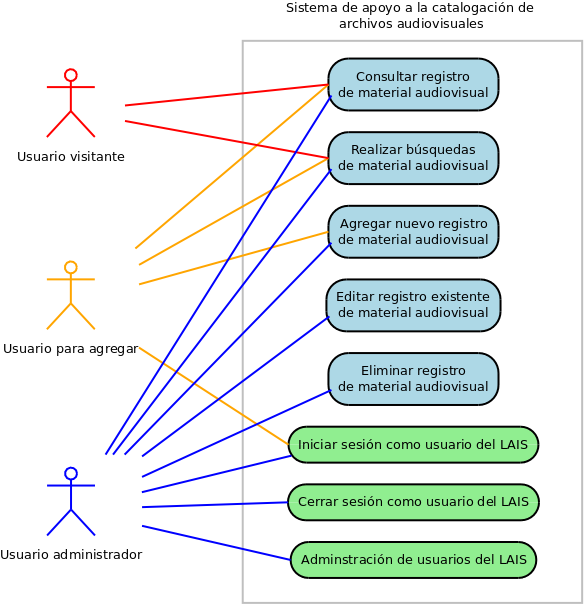
\includegraphics[width=0.7\textwidth]{CasosDeUso.png}
		\caption{Diagrama de casos de uso}
		\label{fig:caso_de_uso}
	\end{figure}
\end{frame}

\section{Acerca del desarrollo de software}
\begin{frame}
	\frametitle{Acerca del desarrollo de software}
	\framesubtitle{Consideraciones}
	Para el tipo de sistema que se desea desarrollar es recomendable tomar en cuenta los siguientes aspectos:
	\begin{itemize}
		\item Arquitectura Modelo-Vista-Controlador
		\item Sistema Manejador de Contenido
		\item Documentación asociada e ingeniería de software
	\end{itemize}
\end{frame}

\begin{frame}
	\frametitle{Acerca del desarrollo de software}
	\framesubtitle{Arquitectura Modelo-Vista-Controlador (MVC)}
	Es un \textbf{patrón de arquitectura} de software para implementar interfaces de usuario que divide a la aplicación de software en tres partes interconectadas para separar la representación interna de la información de la manera en que ésta es presentada al usuario.
	
	\begin{figure}[H]
		\centering
		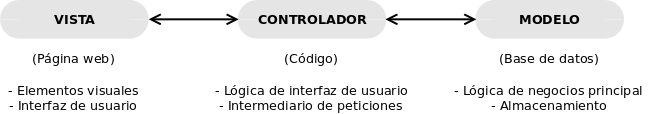
\includegraphics[keepaspectratio=true,width=\linewidth]{ModeloVistaControlador.png}
		\caption{Componentes y su significado en la arquitectura MVC}
		\label{fig:mvc}
	\end{figure}
\end{frame}

\begin{frame}
	\frametitle{Acerca del desarrollo de software}
	\framesubtitle{Sistema Manejador de Contenido (CMS)}
	Aplicación de cómputo que permite \textbf{publicar}, \textbf{editar}, \textbf{modificar} y \textbf{eliminar} contenido desde una interfaz principal. Cumple con dos propósitos principales:
	\begin{itemize}
		\item Permitir a un usuario agregar, modificar y eliminar contenido desde un sitio web sin la intervención de un administrador o programador.
		\item Compilar o almacenar información y actualizar el sitio web.
	\end{itemize}
\end{frame}

\begin{frame}
	\frametitle{Acerca del desarrollo de software}
	\framesubtitle{Documentación asociada e ingeniería de software}
	La ingeniería de software es el estudio y aplicación de la ingeniería al diseño, desarrollo y mantenimiento del software. La documentación generada a partir de esta disciplina \textbf{ayudará} tanto a los usuarios como al equipo de trabajo, \textbf{entender} el funcionamiento del software desarrollado ya sea para su uso, modificación o discusión.
\end{frame}

\section{Selección de tecnologías}
\begin{frame}
	La selección de tecnologías está orientada en utilizar herramientas y estándares ampliamente aceptados y probados:
	\begin{description}
		\item[MySQL] Sistema manejador de bases de datos.
		\item[MySQL Workbench] Herramienta de apoyo a la administración de la base de datos.
		\item[PHP] Lenguaje de programación orientado a servidores (para realizar conexiones a la base).
		\item[AngularJS] Framework para aplicaciones web que brinda la arquitectura modelo-vista-controlador (MVC).
		\item[HTML5] Lenguaje para la creación de la interfaz web (páginas web).
		\item[Bootstrap] Biblioteca adicional para diseño web responsivo.
		\item[Javascript] Lenguaje de programación auxiliar para manejor de eventos.
		\item[jQuery] Biblioteca auxilar para manipulación de páginas web.
	\end{description}
\end{frame}

\section{Diseño de la base de datos}
\begin{frame}
	\frametitle{Diseño de la base de datos}
	Las \textbf{tablas} y los \textbf{campos} (\textbf{columnas}) que lo conforman están basadas en la descripción archivística existente en hojas de cálculo que hasta el momento han sido el modelo a seguir para la catalogación archivística.
\end{frame}

\begin{frame}
	\begin{figure}[H]
		\centering
		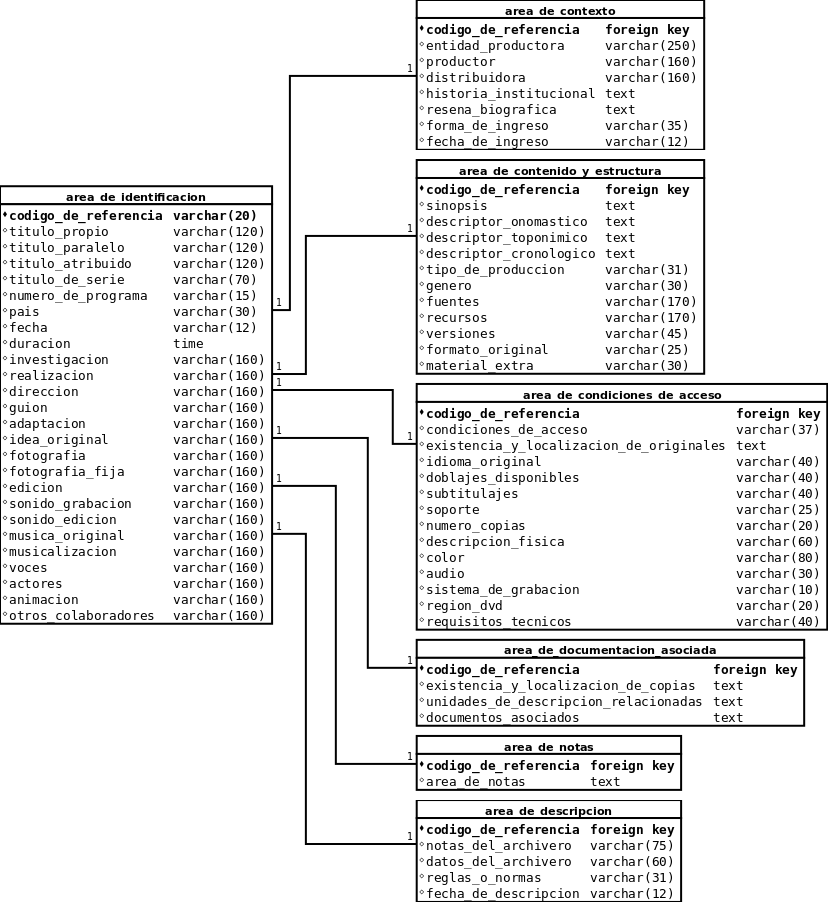
\includegraphics[keepaspectratio=true,scale=0.2]{EntidadRelacion.png}
		\caption{Diagrama Entidad-Relación que muestra el diseño de la base de datos}
		\label{fig:entidad_relacion}
	\end{figure}
\end{frame}

\section{Prototipos}
\begin{frame}
	\frametitle{Prototipos}
	Los prototipos son borradores o sugerencias de diseño previas al desarrollo de una interfaz. El objetivo es que los usuarios puedan dar sus opiniones al respecto para modificar aspectos de diseño en favor de la eficiencia, mejor manejo o un estilo visual más adecuado de la interfaz.
\end{frame}

\begin{frame}
	\begin{figure}[H]
		\centering
		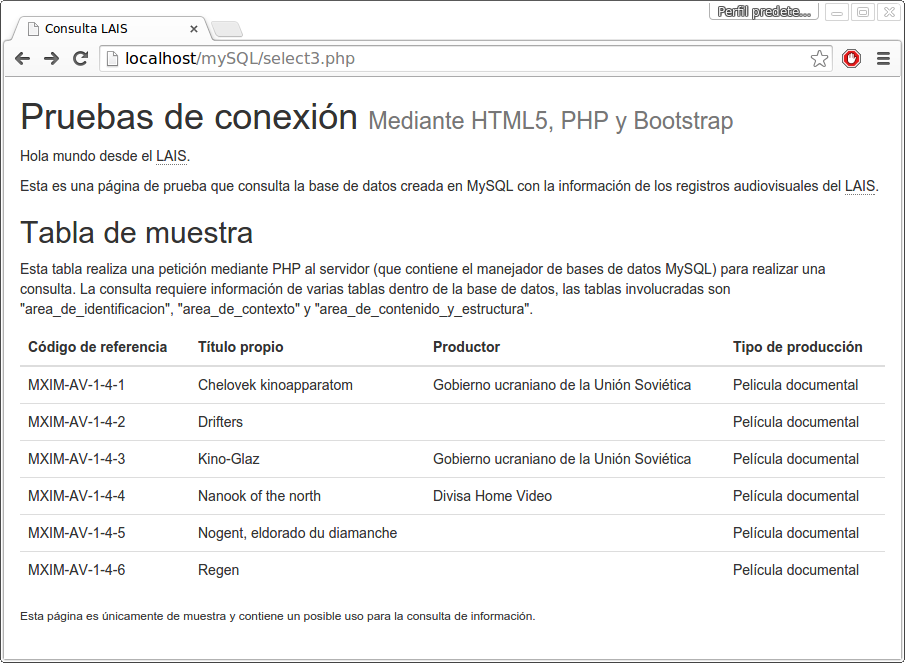
\includegraphics[keepaspectratio=true,width=\linewidth]{Prototipo_01.png}
		\label{fig:prueba_conexion}
	\end{figure}
\end{frame}

%\begin{frame}
%	\begin{figure}[H]
%		\centering
%		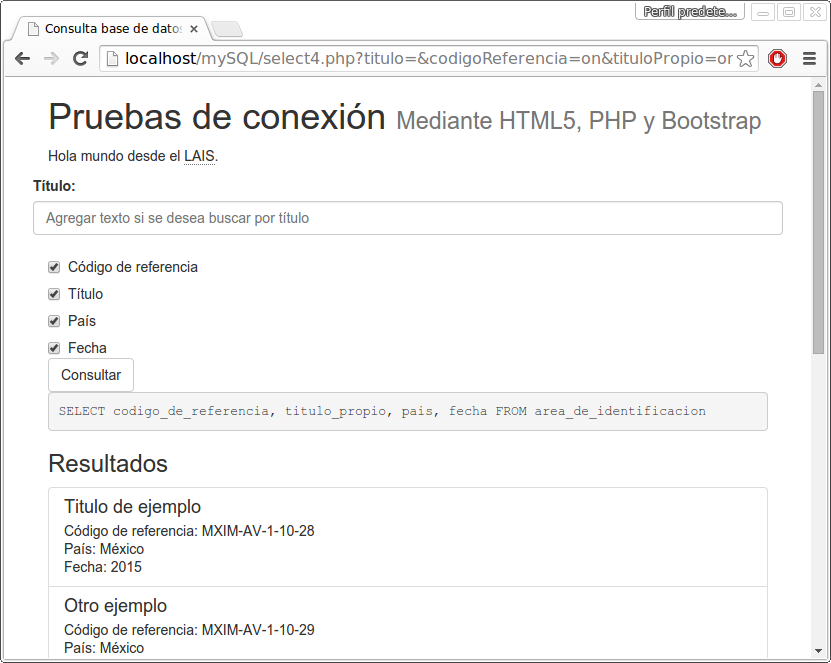
\includegraphics[keepaspectratio=true,width=\linewidth]{Prototipo_02.png}
%		\label{fig:prueba_formulario}
%	\end{figure}
%\end{frame}

%\begin{frame}
%	\begin{figure}[H]
%		\centering
%		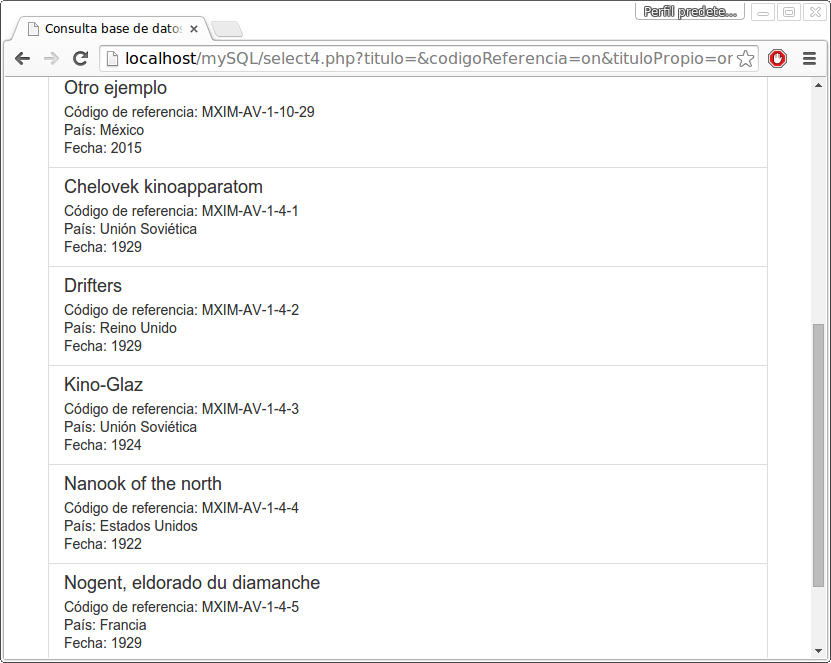
\includegraphics[keepaspectratio=true,width=\linewidth]{Prototipo_03.png}
%		\label{fig:prueba_formulario_2}
%	\end{figure}
%\end{frame}

\begin{frame}
	\begin{figure}[H]
		\centering
		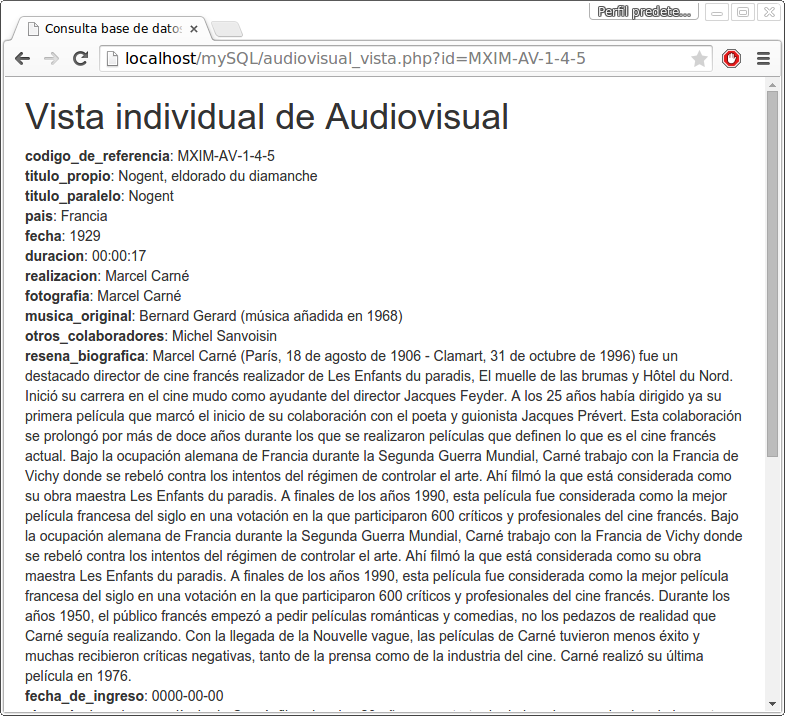
\includegraphics[keepaspectratio=true,width=\linewidth]{Prototipo_04.png}
		\label{fig:vista_audiovisual}
	\end{figure}	
\end{frame}

%\begin{frame}
%	\begin{figure}[H]
%		\centering
%		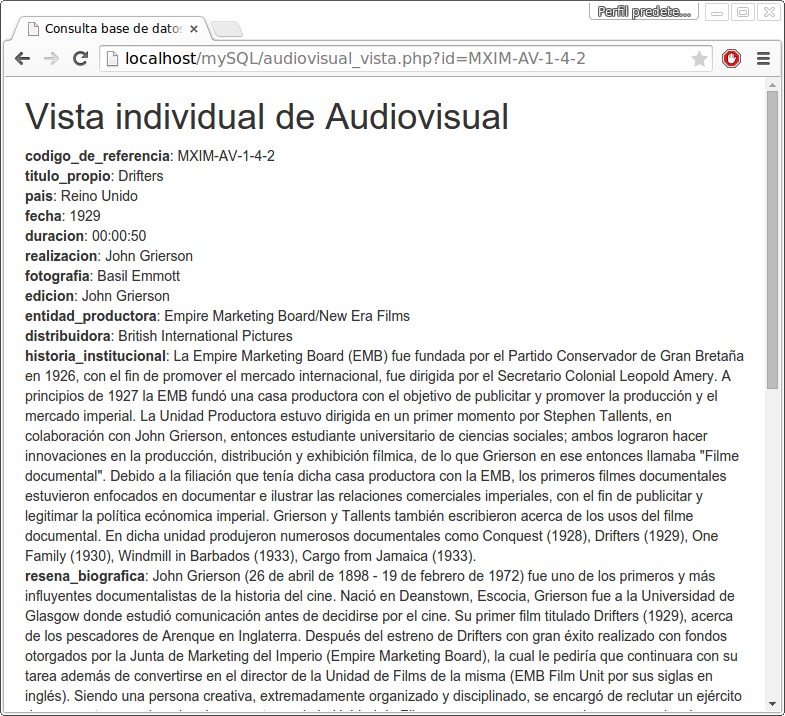
\includegraphics[keepaspectratio=true,width=\linewidth]{Prototipo_05.png}
%		\label{fig:prueba_formulario_2}
%	\end{figure}	
%\end{frame}

\begin{frame}
	\begin{figure}[H]
		\centering
		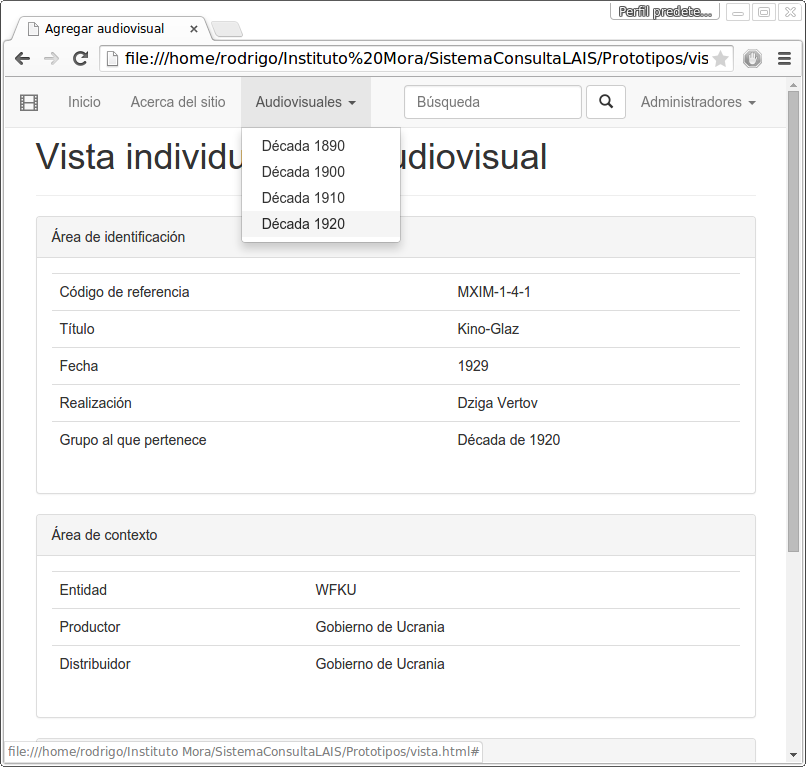
\includegraphics[keepaspectratio=true,width=\linewidth]{Prototipo_06.png}
		\label{fig:disenio_principal}
	\end{figure}	
\end{frame}

\begin{frame}
	\begin{figure}[H]
		\centering
		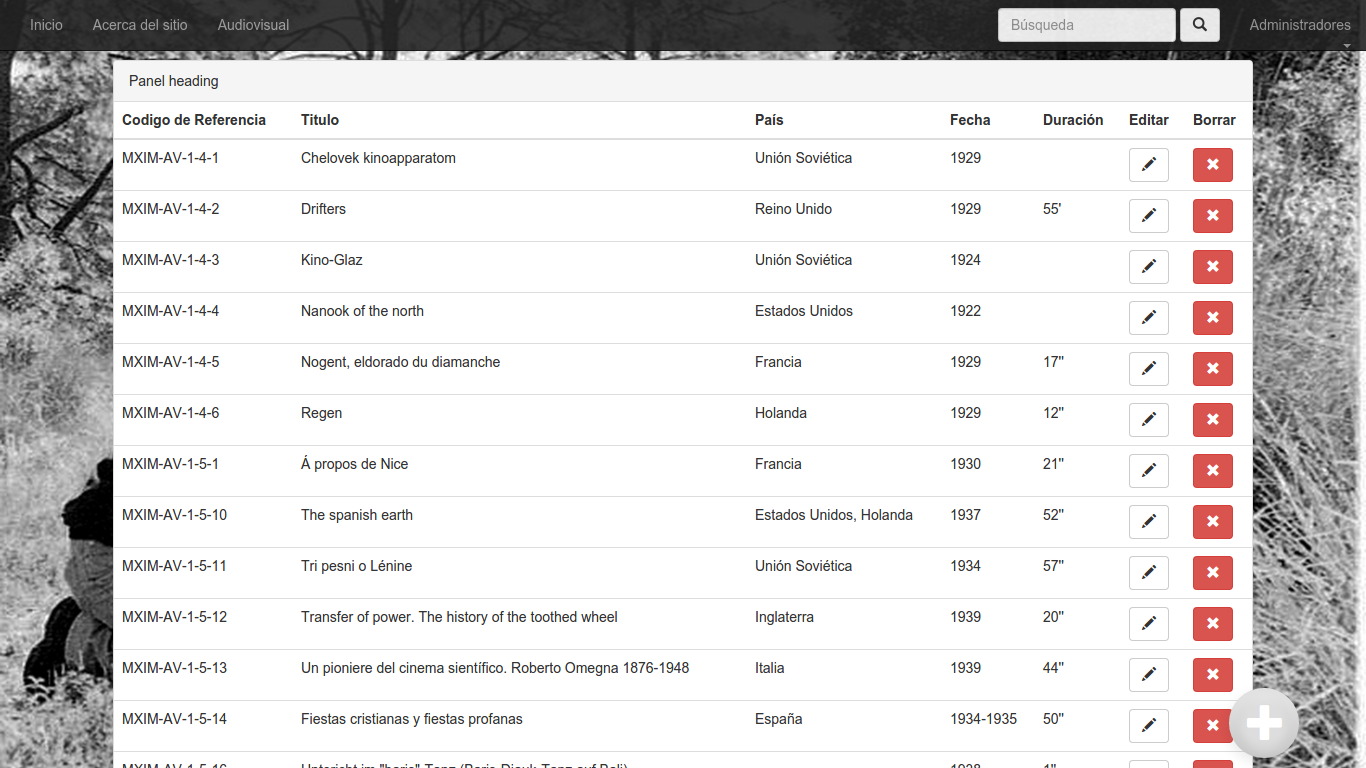
\includegraphics[keepaspectratio=true,width=\linewidth]{Prototipo_07.png}
		\caption{Vista actual del sistema}
		\label{fig:protipo_angular}
	\end{figure}	
\end{frame}

\begin{frame}
	\begin{figure}[H]
		\centering
		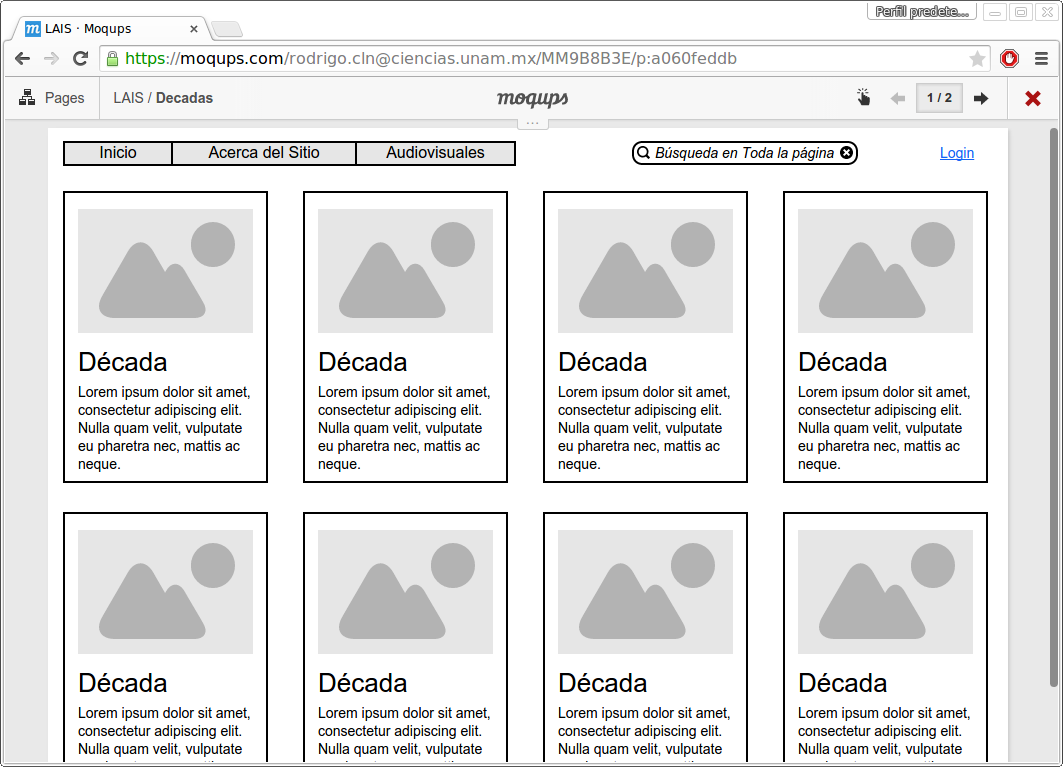
\includegraphics[keepaspectratio=true,width=\linewidth]{Prototipo_08.png}
		\caption{Sugerencia de vista por década}
		\label{fig:protipo_angular}
	\end{figure}	
\end{frame}

\begin{frame}
	\begin{figure}[H]
		\centering
		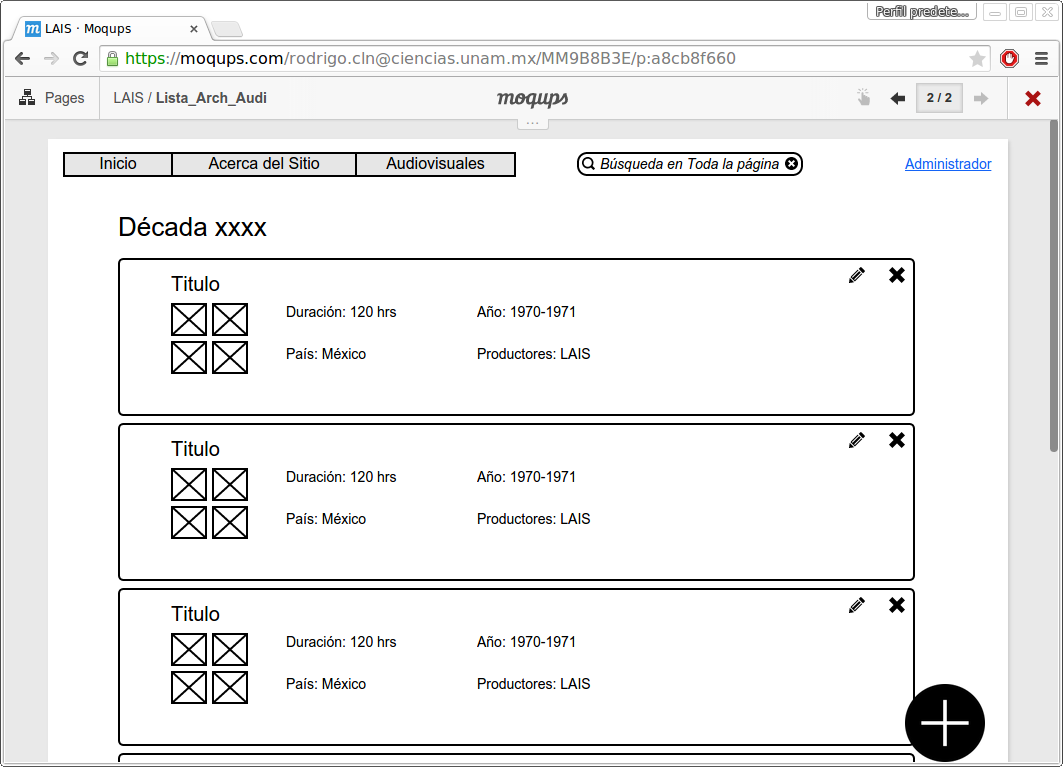
\includegraphics[keepaspectratio=true,width=\linewidth]{Prototipo_09.png}
		\caption{Sugerencia de vista por audiovisuales}
		\label{fig:protipo_angular}
	\end{figure}	
\end{frame}

\section{Observaciones sobre el formulario}
\begin{frame}
	\frametitle{Observaciones sobre el formulario}
	\framesubtitle{Estandarización}
	Para lograr la máxima representatividad de información útil para los usuarios y para los sistemas de cómputo de los archivos audiovisuales, es necesario incluir \textbf{reglas adicionales} al ``Manual de Catalogación del Acervo Documental en Video para la Serie de Documentales en Video del Laboratorio Audiovisual de Investigación Social del Instituto Mora''
\end{frame}

\begin{frame}
	\frametitle{Recomendaciones de catalogación}
	\framesubtitle{Tipos de datos}
	\begin{description}
		\item[Fecha] \hfill \\
			Usar solamente el formato de años o lapso de años. Ejemplo: 1956, 1948-1949. Evitar usar palabras (siglo XIX) u aproximaciones (1992-1993 aprox.).
		\item[Fecha de ingreso] \hfill \\
			Usar el formato día/mes/año o solamente el año. Ejemplo: 31/10/2012 ó 1999. Evitar cambiar el orden por el estándar americano mes/día/año.
		\item[Fecha de descripción] \hfill \\
			Usar el formato estricto día/mes/año. Evitar escribir "Última modificación" junto a la fecha.
	\end{description}
\end{frame}

\begin{frame}
	\frametitle{Recomendaciones de catalogación}
	\framesubtitle{Tipos de datos}
	\begin{description}
		\item[Campos con múltiples nombres] \hfill \\
			Es cómun incluir varios nombres en los siguientes campos: Investigación, Realización, Dirección, Guión, Adaptación, Idea Original, Fotografía, Fotografía fija, Edición, Grabación, Edición, Original, Musicalización, Voces, Actores, Animación, Otros colaboradores, Entidad productora, Productor, Distribuidora, Datos del Archivero.
			
			Debido a eso se recomienda separar cada persona o entidad únicamente mediante el símbolo de coma (,) y evitar usar algún otro separador como diagonal (/), la preposición \textit{y}, guiones (--), punto y coma (;) o cualquier otro símbolo.
	\end{description}
\end{frame}

\begin{frame}
	\frametitle{Recomendaciones de catalogación}
	\framesubtitle{Tipos de datos}
	\begin{description}
		\item[Especificación de rol] \hfill \\
			En campos como \textit{Otros colaboradores} se suele especificar el trabajo de una persona. Por ejemplo: Voz secundaria: Rodrigo Colín.
			
			En estos casos se recomienda utilizar dos puntos (:) para separar el rol específico del nombre. Y separar con comas de la misma manera que se mencionó anteriormente.
	\end{description}
\end{frame}

\begin{frame}
	\frametitle{Recomendaciones de catalogación}
	\framesubtitle{Tipos de datos}
	\begin{description}
		\item[Campos con sugerencias] \hfill \\
			Aplica para los campos Forma de ingreso, Tipo de producción y Condiciones de acceso, en donde se recomienda utilizar los valores que se muestran. Sin embargo, el campo queda abierto por si se requiere escribir algún otro valor distinto a los mostrados.
		\item[Campos estrictos] \hfill \\
			Los campos de Fuentes y Recursos son los únicos campos estrictos y es por eso que se deben seleccionar únicamente los valores que se muestran.
	\end{description}
\end{frame}

\section{Próximo desarrollo}
\begin{frame}
	\frametitle{Próximo desarrollo}
	\framesubtitle{Tareas pendientes (por orden de prioridad)}
	\begin{itemize}
		\item Dar funcionalidad para realizar búsquedas.
		\item Agregar manejo de identificación y permisos (login).
		\item Incluir imágene(s) para cada audiovisual.
		\item Depurar la información de las hojas de cálculo para incluir en la base de datos.
		\item Configurar el servidor.
	\end{itemize}
\end{frame}

\section{Conclusión}
\begin{frame}
	\frametitle{Conclusiones}
	\begin{itemize}
		\item Se logró implementar satisfactoriamente la parte principal del sistema que cumple con la arquitectura MVC y permite las operaciones principales de un manejador de contenido (CMS). Se continuará el desarrollo del sistema para integrar más componentes y vistas necesarios.
		\item Se aportan recomendaciones a la catalogación de archivos audiovisuales estandarizar los datos de los archivos audiovisuales para su uso práctico con usuario y en sistemas computacionales.
		\item Durante el desarrollo, siempre tener como objetivo la creación un sistema capaz de organizarse y administrarse de manera simple por parte de los usuarios del LAIS sin la necesidad de intervención de los programadores.
		\item Crear y mantener una base de datos estandarizada para reutilizar esa información mediante un manejo semántico de contenido (siguiente proyecto a desarrollar).
	\end{itemize}
\end{frame}

\begin{frame}
	\begin{center}
		GRACIAS POR SU TIEMPO.
		
		
\includegraphics{scientistapprovedfutura.png}
	\end{center}
\end{frame}

\end{document}